% Diagram 1/3 — Overall generation workflow (snake layout, slide-friendly 16:9)
% Cloudflare Workers (Hono) + Cloudflare Queues + Workers AI + Cartesia.
% Storage layout -> storage.tex   ·   DB schema -> database.tex
% Build:  pdflatex workflow.tex
\documentclass[border=14pt]{standalone}
\usepackage[T1]{fontenc}
\usepackage{lmodern}
\usepackage{tikz}
\usetikzlibrary{positioning, arrows.meta, shapes.geometric, backgrounds, fit, calc}

\definecolor{wkBlue}{HTML}{1D4E89}
\definecolor{wkBlueBg}{HTML}{E8F0FB}
\definecolor{qOrange}{HTML}{C75B12}
\definecolor{stTeal}{HTML}{0E6B6B}
\definecolor{stTealBg}{HTML}{DDF1F1}
\definecolor{dbGreen}{HTML}{2E6F40}
\definecolor{dbGreenBg}{HTML}{E5F2E8}
\definecolor{extPurple}{HTML}{5B2A86}
\definecolor{extPurpleBg}{HTML}{EFE6F7}
\definecolor{todoGray}{HTML}{6B7280}
\definecolor{inkGray}{HTML}{475569}
\definecolor{entryInk}{HTML}{334155}

\newcommand{\sub}[1]{{\scriptsize\textcolor{inkGray}{#1}}}
\newcommand{\file}[1]{{\scriptsize\ttfamily\textcolor{inkGray}{#1}}}

\begin{document}
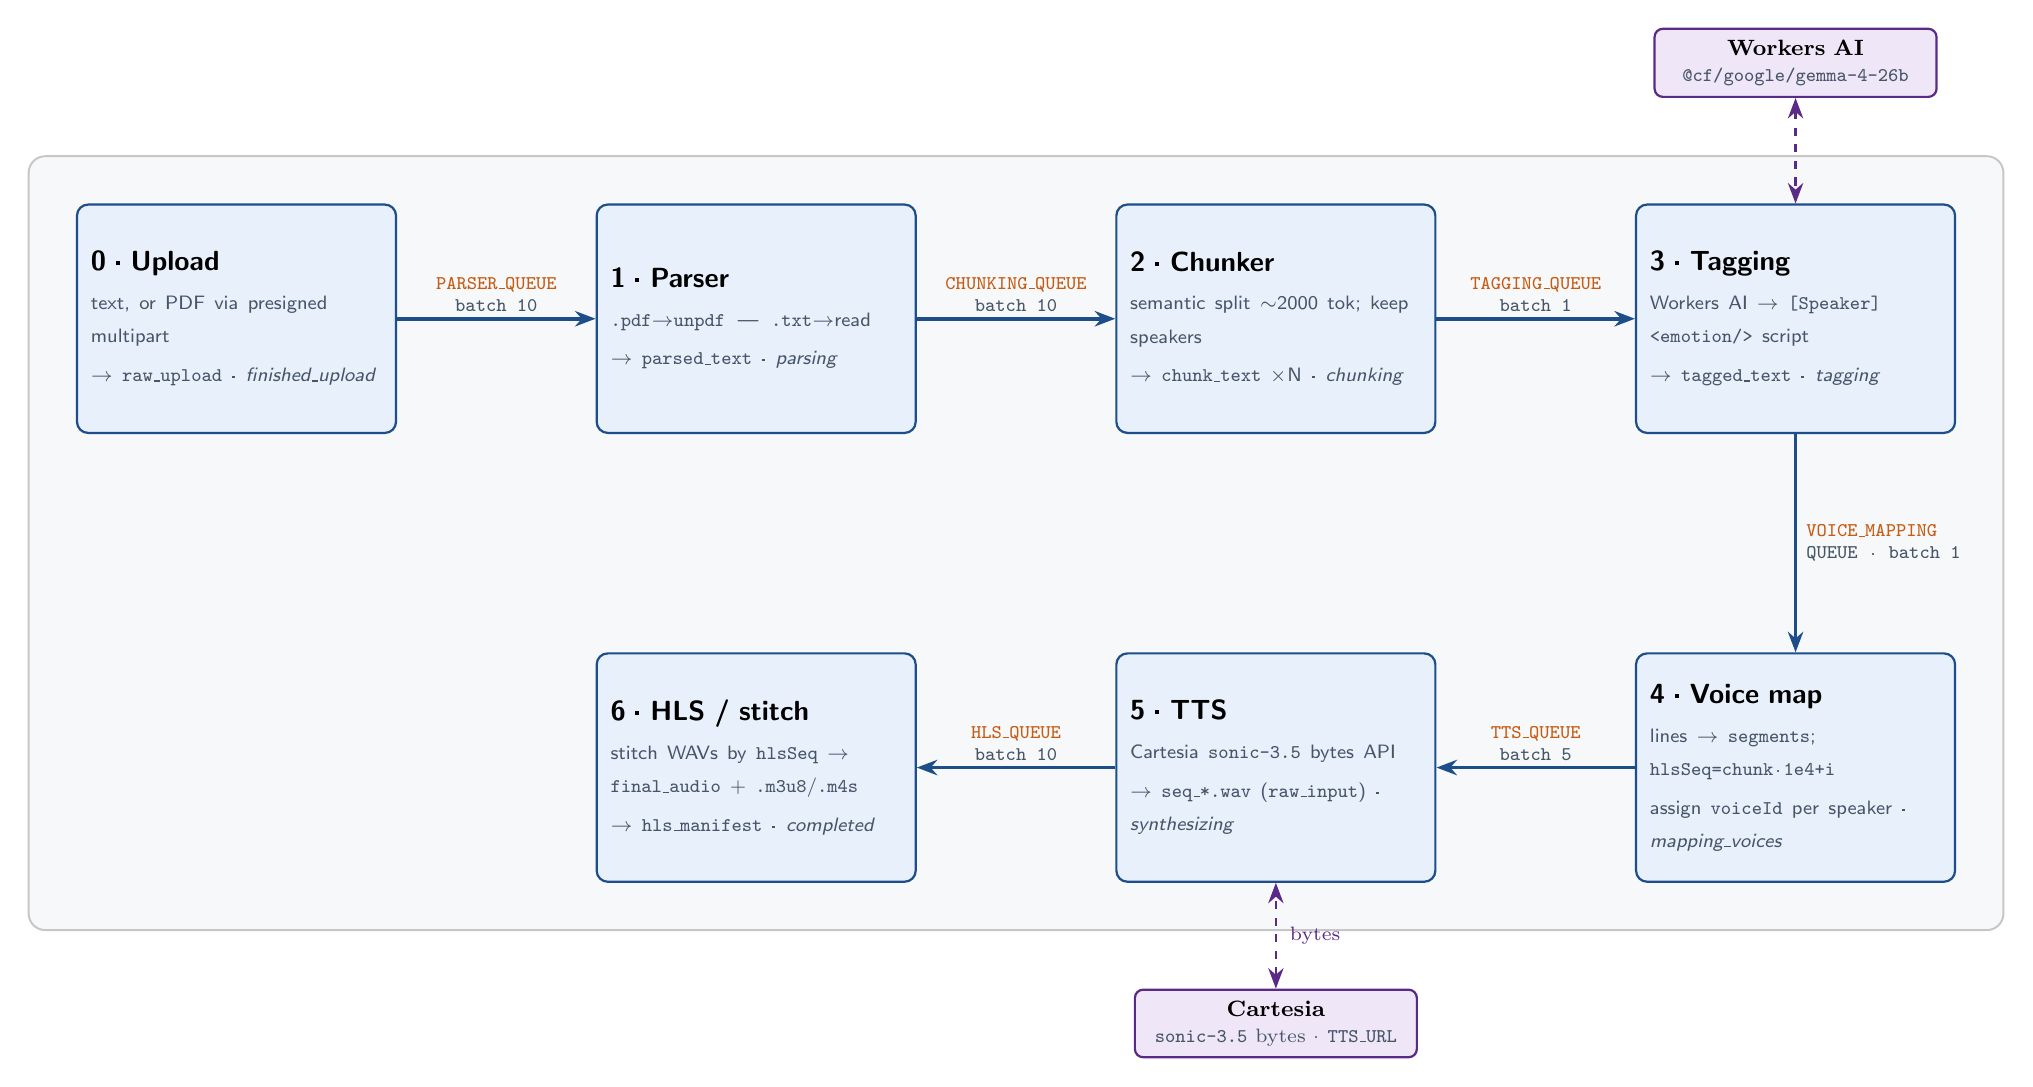
\begin{tikzpicture}[
  font=\sffamily,
  >={Stealth[length=2.6mm]},
  stage/.style={rectangle, rounded corners=4pt, draw=wkBlue, line width=0.8pt,
                fill=wkBlueBg, align=left, inner sep=5pt, text width=37mm, minimum height=29mm},
  entry/.style={rectangle, rounded corners=4pt, draw=entryInk, line width=1pt,
                fill=gray!12, align=left, inner sep=5pt, text width=37mm, minimum height=29mm},
  todo/.style={rectangle, rounded corners=4pt, draw=todoGray, dashed, line width=1pt,
               fill=gray!7, align=left, inner sep=5pt, text width=37mm, minimum height=29mm, text=todoGray},
  ext/.style={rectangle, rounded corners=3pt, draw=extPurple, line width=0.8pt,
              fill=extPurpleBg, align=center, inner sep=4pt, text width=33mm, font=\footnotesize},
  note/.style={rectangle, rounded corners=4pt, draw=gray!50, line width=0.7pt,
               fill=gray!4, align=left, inner sep=6pt, font=\scriptsize},
  flow/.style={->, line width=1.3pt, draw=wkBlue},
  flowtodo/.style={->, line width=1.2pt, draw=todoGray, dashed},
  extflow/.style={<->, line width=0.8pt, draw=extPurple, dashed},
  qlab/.style={font=\scriptsize\ttfamily, text=qOrange, align=center, inner sep=2pt},
  panelbg/.style={rounded corners=6pt, draw=gray!45, line width=0.7pt, fill=none},
]

% ===== Pipeline — row 1 (L->R): 0,1,2,3 =====================================
\node[stage] (client) at (0,0)
  {\textbf{0 · Upload}\\[2pt]
   \sub{text, or PDF via presigned multipart}\\[2pt]
   \sub{$\to$ \texttt{raw\_upload} · \textit{finished\_upload}}};
\node[stage] (parser) at (6.6,0)
  {\textbf{1 · Parser}\\[2pt]
   \sub{\texttt{.pdf}$\to$\texttt{unpdf} \,|\, \texttt{.txt}$\to$read}\\[2pt]
   \sub{$\to$ \texttt{parsed\_text} · \textit{parsing}}};
\node[stage] (chunker) at (13.2,0)
  {\textbf{2 · Chunker}\\[2pt]
   \sub{semantic split $\sim$2000 tok; keep speakers}\\[2pt]
   \sub{$\to$ \texttt{chunk\_text} ×N · \textit{chunking}}};
\node[stage] (tagging) at (19.8,0)
  {\textbf{3 · Tagging}\\[2pt]
   \sub{Workers AI $\to$ \texttt{[Speaker] <emotion/>} script}\\[2pt]
   \sub{$\to$ \texttt{tagged\_text} · \textit{tagging}}};

% ===== Pipeline — row 2 (R->L): 4,5,6 =======================================
\node[stage] (vmap) at (19.8,-5.7)
  {\textbf{4 · Voice map}\\[2pt]
   \sub{lines $\to$ \texttt{segments}; \texttt{hlsSeq=chunk·1e4+i}}\\[2pt]
   \sub{assign \texttt{voiceId} per speaker · \textit{mapping\_voices}}};
\node[stage] (tts) at (13.2,-5.7)
  {\textbf{5 · TTS}\\[2pt]
   \sub{Cartesia \texttt{sonic-3.5} bytes API}\\[2pt]
   \sub{$\to$ \texttt{seq\_*.wav} (\texttt{raw\_input}) · \textit{synthesizing}}};
\node[stage] (hls) at (6.6,-5.7)
  {\textbf{6 · HLS / stitch}\\[2pt]
   \sub{stitch WAVs by \texttt{hlsSeq} $\to$ \texttt{final\_audio} + \texttt{.m3u8}/\texttt{.m4s}}\\[2pt]
   \sub{$\to$ \texttt{hls\_manifest} · \textit{completed}}};

% ---- flow arrows + queue labels ----
\draw[flow] (client) -- (parser) node[qlab, midway, above] {PARSER\_QUEUE\\\sub{batch 10}};
\draw[flow] (parser) -- (chunker) node[qlab, midway, above] {CHUNKING\_QUEUE\\\sub{batch 10}};
\draw[flow] (chunker) -- (tagging) node[qlab, midway, above] {TAGGING\_QUEUE\\\sub{batch 1}};
\draw[flow] (tagging) -- (vmap) node[qlab, midway, right, align=left] {\,VOICE\_MAPPING\\\,\sub{QUEUE · batch 1}};
\draw[flow] (vmap) -- (tts) node[qlab, midway, above] {TTS\_QUEUE\\\sub{batch 5}};
\draw[flow] (tts) -- (hls) node[qlab, midway, above] {HLS\_QUEUE\\\sub{batch 10}};

% ===== External services =====================================================
\node[ext] (wai) at (19.8,3.25) {\textbf{Workers AI}\\\sub{\texttt{@cf/google/gemma-4-26b}}};
\node[ext] (cart) at (13.2,-8.95) {\textbf{Cartesia}\\\sub{\texttt{sonic-3.5} bytes · \texttt{TTS\_URL}}};
\draw[extflow] (wai.south) -- (tagging.north) node[midway, right, font=\scriptsize, text=extPurple] {};
\draw[extflow] (cart.north) -- (tts.south) node[midway, right, font=\scriptsize, text=extPurple] {\,bytes};

% ===== Title (centered above row 1) =========================================
% \node[font=\sffamily\bfseries\Large] (title) at (9.9,5.55) {Audiobook generation workflow};
% \node[below=0.5mm of title, font=\sffamily, text=inkGray]
%   {single \texttt{queue()} consumer fans out by queue name — one Cloudflare Worker, six stages};

% % ===== Bottom note band =====================================================
% \node[note, anchor=north west, text width=74mm] (contract) at (-1.85,-11.0)
%   {\textbf{\textcolor{wkBlue}{Per-stage worker contract}} \file{queue.ts}\\[2pt]
%    1.\ \texttt{getDb(HYPERDRIVE)} · \texttt{storage.getInstance(env)} \quad
%    2.\ validate body; \texttt{ack()} poison msgs\\
%    3.\ \texttt{update audiobooks.status} \quad
%    4.\ work · \texttt{putObject} · insert \texttt{assets}/\texttt{segments}\\
%    5.\ \texttt{env.NEXT\_QUEUE.send()} \quad 6.\ \texttt{ack()} \quad
%    7.\ on error \texttt{status=failed} + \texttt{retry()}};
% \node[note, anchor=north west, text width=57mm, fill=stTealBg, draw=stTeal] (psto) at (6.0,-11.0)
%   {\textbf{\textcolor{stTeal}{Object storage}} (R2 / Supabase)\\[2pt]
%    every stage reads/writes artifacts via the storage abstraction.
%    \textbf{Buckets \& keys $\to$ \texttt{storage.tex}}};
% \node[note, anchor=north west, text width=57mm, fill=dbGreenBg, draw=dbGreen] (pdb) at (12.7,-11.0)
%   {\textbf{\textcolor{dbGreen}{Postgres (Supabase)}} · Drizzle / Hyperdrive\\[2pt]
%    each stage updates \texttt{audiobooks.status} and records \texttt{assets} / \texttt{segments}.
%    \textbf{Schema $\to$ \texttt{database.tex}}};

% ===== Worker swimlane background ===========================================
\begin{scope}[on background layer]
  \node[panelbg, fill=wkBlue!4,
        fit=(client)(parser)(chunker)(tagging)(vmap)(tts)(hls), inner sep=6mm] (workerbox) {};
\end{scope}

% % ===== Legend ===============================================================
% \node[anchor=north west, align=left, font=\scriptsize, text=inkGray,
%       draw=gray!40, rounded corners=3pt, inner sep=5pt] (legend) at (-1.85,-10.8)
%   {\textbf{Legend}\quad
%    \tikz\draw[entryInk, line width=1pt, fill=gray!12, rounded corners=2pt] (0,0) rectangle (0.45,0.22);\ HTTP route \quad
%    \tikz\draw[wkBlue, line width=0.8pt, fill=wkBlueBg, rounded corners=2pt] (0,0) rectangle (0.45,0.22);\ queue worker \quad
%    \tikz{\draw[flow] (0,0.09) -- (0.6,0.09); \node[qlab] at (0.3,0.32){QUEUE};}\ Cloudflare Queue hop \quad
%    \tikz\draw[extPurple, dashed, <->] (0,0.09) -- (0.5,0.09);\ external call};

\end{tikzpicture}
\end{document}
